\documentclass[12pt]{article}
\usepackage{amsmath}
\usepackage{amssymb}
\usepackage{graphicx}
\usepackage[margin=1in]{geometry}
\usepackage{parskip}

\begin{document}

\noindent
\begin{minipage}[c]{0.25\textwidth}
    
\includegraphics[width=1\linewidth]{iiitb_logo.jpg}
\end{minipage}
\hfill
\begin{minipage}[c]{0.35\textwidth}
    \raggedleft
    \textbf{Name:} Shaik Ameen\\
    \textbf{ID:} COMETFWC074\\
    \textbf{Date:} \today
\end{minipage}

\vspace{0.2cm}
\hrule
\vspace{0.4cm}

\noindent

\textbf{Q.31} \hspace{0.3cm} What is the boolean expression for the output $f$ of the combinational logic circuit of NOR gates given below?

\vspace{0.5cm}

\begin{center}
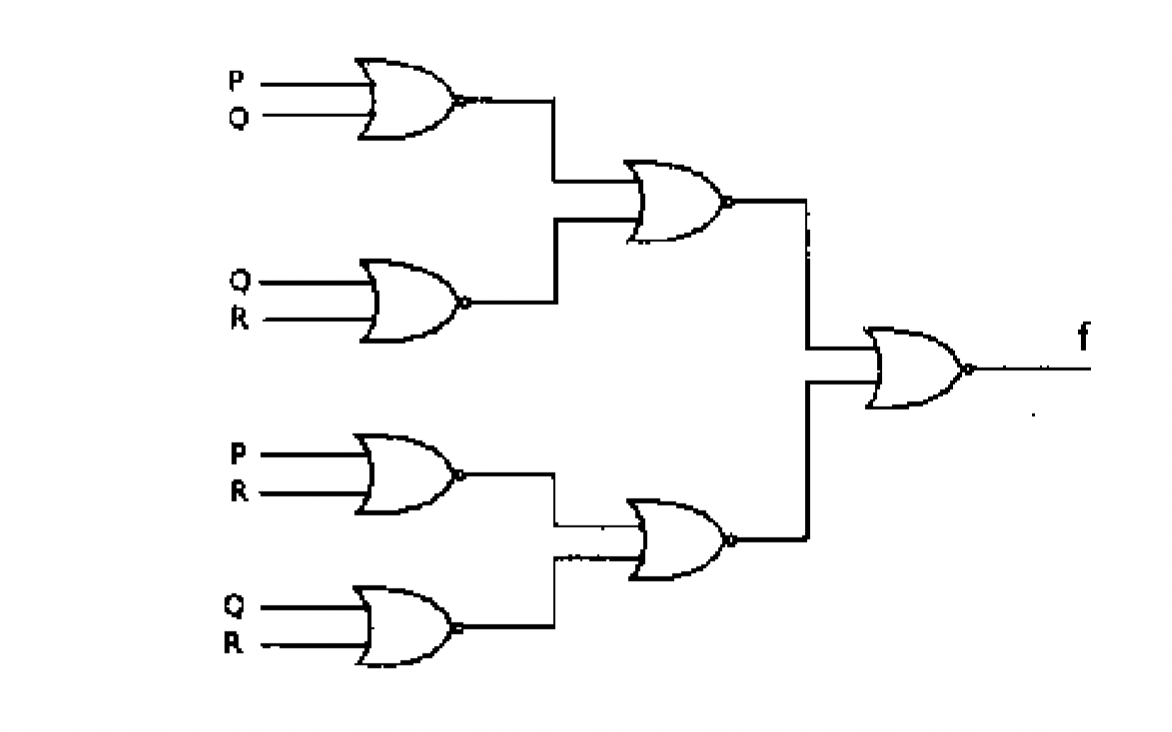
\includegraphics[width=0.6\textwidth]{q31_circuit.png}
\end{center}

\vspace{0.3cm}

\begin{center}
(A) $\overline{Q+R}$ \hspace{1.5cm}
(B) $\overline{P+Q}$ \hspace{1.5cm}
(C) $\overline{P+R}$ \hspace{1.5cm}
(D) $\overline{P+Q+R}$
\end{center}

\vspace{0.5cm}

{\large \textbf{Solution}}

\vspace{0.4cm}

Since all the gates in the circuit are NOR gates,

$$
\text{NOR Gate Output} = \overline{A+B}
$$

Let the outputs of the first stage NOR gates be

\begin{align*}
X_1 &= \overline{P+Q} \\
X_2 &= \overline{Q+R}
\end{align*}

These outputs are applied to another NOR gate.

\begin{align*}
Y_1 
&= \overline{X_1 + X_2} \\
&= \overline{\overline{P+Q} + \overline{Q+R}}
\end{align*}

Using DeMorgan's law,

$$
Y_1 = (P+Q)(Q+R)
$$

Similarly, for the lower section,

\begin{align*}
X_3 &= \overline{P+R} \\
X_4 &= \overline{Q+R}
\end{align*}

Their NOR output is

\begin{align*}
Y_2 
&= \overline{X_3 + X_4} \\
&= \overline{\overline{P+R} + \overline{Q+R}}
\end{align*}

Applying DeMorgan's law,

$$
Y_2 = (P+R)(Q+R)
$$

Finally, the outputs $Y_1$ and $Y_2$ are connected to the last NOR gate.

\begin{align*}
f 
&= \overline{Y_1 + Y_2} \\
&= \overline{(P+Q)(Q+R) + (P+R)(Q+R)}
\end{align*}

Simplifying,

$$
f = \overline{P+R}
$$

\vspace{0.4cm}

\begin{center}
\boxed{\textbf{Correct Answer: Option (C) } \overline{P+R}}
\end{center}

\end{document}
